\chapter{Implementación de la PCB\label{sec:Implementacion_PCB}}

En el diseño e implementación de la \acrshort{PCB} es muy importante tener presente que cualquier fallo a nivel de hardware supone una gran pérdida de tiempo y, por lo tanto, dinero. Desde que el diseño es terminado y se manda a producir la placa hasta que esta se recibe transcurre una media de dos semanas . Perder esa cantidad de tiempo por un fallo de diseño a nivel docente supone, en el peor de los casos, no entregar el proyecto en la fecha acordada, pero a nivel empresarial puede significar perder la exclusividad del diseño cuando se compite con otras compañías. 

En el diseño es muy importante revisar cualquier tipo de error con el fin de evitar retrasos en la entrega de proyectos. Una revisión manual puede evitar parte de ellos pero la utilización de una buena herramienta bien configurada contribuye a la realización de esta tarea de una manera más rápida y eficaz. Como ya se ha mencionado en el capítulo \ref{sec:Diseno}, para la realización de este proyecto se ha utilizado la herramienta KiCad, no sólo por ser Software Libre sino porque presenta ciertas ventajas o características muy interesantes:
\begin{itemize}
\item \textbf{Entorno de desarrollo integrado:}
\\Desde la propia herramienta se pueden hacer los esquemáticos, definir los componenes y librerías e, incluso, diseñar y previsualizar la \acrshort{PCB}.
\item \textbf{Multiplataforma:}
\\Disponible en Windows, Linux y Mac OS.
\item \textbf{Respaldado por una gran comunidad} 
\\KiCad tiene una gran comunidad que deja a disposición de los usuarios una documentación muy extensa.
\item \textbf{Constante desarrollo}
\\Se liberan actualizaciones con regularidad.
\end{itemize}

Al abrir la herramienta se carga un gestor de proyectos desde el que se puede gestionar un gran número de elementos.

\begin{figure} [h]
    \centering
    \includegraphics[width=13cm]{Front_end_Kicad}
    \caption{Gestor de proyectos de KiCad}
    \label{fig:Front_end_Kicad}
\end{figure}

Como se puede observar en la imagen, a la izquierda aparecen todos los archivos pertenecientes al proyecto mientras que en la parte superior hay un acceso directo a las distintas partes que componen la herramienta (gestor de esquemáticos, librerías, modelos 3D, etc).

Durante la fase de diseño y realización del esquemático, cada componente fue seleccionado de entre los disponibles preinstalados en KiCad. Aunque los componentes más comunes como son las resistencias o los condensadores se pueden encontrar sin problemas, para trabajar con otros componentes como el ESP ha sido necesario crear una librería propia. Más adelante, cuando las especificaciones de diseño se hayan definido, se enlazará el símbolo que representa cada componente con el elemento físico que estará presente en la \acrshort{PCB}, es decir, su \textit{footprint} y su modelo 3D.

\section{Limitaciones del fabricante\label{sec:ITEAD_PCB}}

El diseño de la \acrshort{PCB} tiene ciertas \textbf{restricciones}, algunas impuestas por el propio diseño del circuito (tipo de componentes, número de pistas, tamaño final, etc.), otras, como las tratadas en esta sección, serán \textbf{impuestas por el propio fabricante de \acrshort{PCB}s}.

La mayoría de empresas fabricantes de PCBs del mercado dejan a disposición de sus clientes un listado de las limitaciones con las que cuentan, garantizando que cualquier diseño que se adecue a ellas será impreso correctamente. 

De entre las disponibles en el mercado se seleccionó la compañía ITEAD por presentar una buena relación prestaciones/precio, un tiempo de impresión y envío bajo y haberse contratado sus servicios con anterioridad.

En su página web \cite{ITEAD_PCB_Limitations}, ITEAD ha preparado una tabla con un resumen de las características con las que se puede contar si se imprime una \acrshort{PCB} en condiciones normales. Dicha tabla se recoge a continuación:

\begin{table} [H]
\centering
\begin{tabular}{|c|c|}
\hline 
\textbf{Característica} & \textbf{Valor} \\
\hline 
Layers &	1 - 4 \\
\hline 
Material & 	FR-4 \\
\hline 
Board Dimension (max) & 	380mm X380mm \\
\hline 
Board Dimension (min) &	10mm X10mm \\
\hline 
Outline Dimension Accuracy &  $\pm$0.2mm \\
\hline 
Board Thickness & 	0.40mm--2.0mm \\
\hline 
Board Thickness Tolerance &	 $\pm$10\% \\
\hline 
Dielectric Separation thickness &	0.075mm--5.00mm \\
\hline 
Conductor Width (min) &	0.15mm (Recommend>8mil) \\
\hline 
Conductor Space (min) &	0.15mm (Recommend>8mil) \\
\hline 
Outer Conductor thickness &	35um \\
\hline 
Inner Conductor thickness &	17um--100um \\
\hline 
Copper to Edge &	>0.3mm \\
\hline 
Plated Component &	 \multirow{2}{*}{0.3mm--6.30mm} \\
Plated via Diameter(Mechanical) & \\
\hline 
Plated Hole Diameter Tolerance(Mechanical) &	0.08mm \\
\hline 
Unplated Hole Diameter Tolerance &	0.05mm \\
\hline 
Hole Space(min) &	0.25mm \\
\hline 
Hole to Edge &	0.4mm \\
\hline 
Annular Ring(min) &	0.15mm \\
\hline 
Solder Resist Type & 	Photosensitive ink \\
\hline 
Solder Resist Color &	Black, Green, White, Blue, Yellow \\
\hline 
Solder Resist Clearance &	0.1mm \\
\hline 
Solder Resist Coverage &	0.1mm \\
\hline 
Plug Hole Diameter &	0.3mm--0.65mm \\
\hline 
Silkscreen line width (mim) &	6mil \\
\hline 
\end{tabular} 
\caption{Restricciones de ITEAD para la fabricación de una PCB}
\label{tab:ITEAD}
\end{table}

Aunque la lista de restricciones parece alta, la mayoría de ellas no supone un problema para un proyecto de estas dimensiones. Para comprobar si esta afirmación es correcta bastará con comprobar si la característica más restrictiva se cumple, es decir, comparar la separación mínima de los pads del módulo Bluetooth con la separación mínima entre conductores, denominada en la tabla \ref{tab:ITEAD} como \textit{Conductor Space}. De acuerdo a su \textit{datasheet}, la separación entre pines de este componente es de 9.84 mil (0.25 mm), valor muy superior a los 8 mil (0.2 mm) recomendados por el fabricante.
\clearpage
Adicionalmente, informan de que la utilización de \textit{Buried vias} y \textit{Blind vias} no es posible por el momento.

\begin{figure} [h]
    \centering
    \includegraphics[width=10cm]{ITEAD_vias}
    \caption{Tipos de vías}
    \label{fig:ITEAD_vias}
\end{figure}

Con toda la información recopilada hasta el momento ya es posible configurar KiCad para forzar que dichas restricciones se cumplan en todo momento. El menú ``\textit{Design Rules}'' permite configurar estos parámetros (ver fig. \ref{fig:Design_rules_general}) así como realizar ciertos ajustes dependiendo de la función que tendrá cada pista (ver fig. \ref{fig:Design_rules_especial}).

\begin{figure}[h]
  \begin{subfigure}[b]{8cm}
   	\centering
    \includegraphics[width=8cm]{Design_rules_1}
    \caption{Condiciones especiales}
    \label{fig:Design_rules_especial}
  \end{subfigure}
  \hfill
  \begin{subfigure}[b]{8cm}
  	\centering
    \includegraphics[width=8cm]{Design_rules_2}
    \caption{Reglas de diseño en KiCad}
    \label{fig:Design_rules_general}
  \end{subfigure}
  \caption{Reglas de diseño en KiCad cumpliendo las restricciones de ITEAD}
  \label{fig:Design_rules}
\end{figure}

\clearpage

\section{Componentes y librerías\label{sec:Componentes_y_librerias}}

Aunque en el esquemático se escogieron los valores de todos los componentes, a la hora de realizar un diseño final hay que tener en cuenta otros muchos parámetros. ¿Qué tamaño tendrá el componente?, ¿cuál será su tolerancia?, ¿qué formato se ajusta mejor, \acrshort{THT} o \acrshort{SMT}? La respuesta a todas estas preguntas acabará definiendo el componente a elegir, su precio y su disponibilidad.

Utilizar componentes en el formato \acrshort{THT} puede suponer una ventaja las primeras veces que se realiza una soldadura o al trabajar con electrónica de potencia. En ambos casos se aprovecha el grosor del conector y el hecho de que atraviese la placa para dar mayor comodidad al técnico y disminuir la resistividad de la unión respectivamente. 
\\Por desgracia, al trabajar con electrónica digital o analógica que no involucra alta potencia, la utilización de dichos componentes limita el diseño e impone restricciones que mediante \acrshort{SMT} se evitan con relativa facilidad. Un claro ejemplo es la imposibilidad de enrutar pistas bajo los conectores de dichos componentes \acrshort{THT}.
\\A lo largo del diseño de la \acrshort{PCB} se seleccionará en la medida de lo posible componentes en su formato \textbf{\acrshort{SMT}} ya que además introducen menos ruido en el circuito.

Por simplicidad y comodidad se ha escogido trabajar con una tamaño estándar de \textbf{0603 con medidas de 0.063'' x 0.031'' (1,6 mm x 0,8 mm)} ya que, por un lado permiten su manejo y soldado sin necesidad de herramientas especiales y, por otro, son medidas muy comunes facilitando la localización de componentes así como de distribuidores primarios y secundarios.

\begin{figure} [h]
    \centering
    \includegraphics[width=5cm]{0603}
    \caption{Resistencia en formato 0603 \cite{Imagen_0603}}
    \label{fig:0603}
\end{figure}

\subsection{Asignación de \textit{footprint}\label{sec:Enlazado}}

Tras decidir el tamaño de los componentes se debe \textbf{enlazar} cada uno de los \textbf{símbolos} presentes en el \textbf{esquemático} que se generó al comienzo del proyecto su \textbf{\textit{footprint}} correspondiente. Adicionalmente pueden añadirse \textbf{modelos 3D} para una visualización más realista del acabado final.

Si bien el segundo elemento no es normalmente necesario, el primero resulta imprescindible pues contiene información básica sobre el componente (número de pads y conexiones, tamaño real, serigrafías, etc). 

Como ya se ha mencionado anteriormente, KiCad se caracteriza por tener una gran comunidad que lo respalda. Esto se traduce en que la mayoría de los componentes del mercado ya han sido incluidos en \textbf{librerías de código abierto} disponibles en Internet, lo cual supone un ahorro considerable de tiempo de cara a este o futuros proyectos. 
Por desgracia esto no es siempre suficiente por lo que KiCad ha sido diseñado para, en caso de ser necesario, crear una librería en la que almacenar los \textit{footprints}, serigrafías y \textbf{modelos 3D propios}, conteniendo las \textbf{herramientas con las que crear o editar} uno ya existente para adaptarlo a las necesidades del proyecto.

\begin{figure} [h]
    \centering
    \includegraphics[width=16cm]{Footprint_ESP}
    \caption{\textit{Footprint }modificado para adaptarlo al ESP12-E}
    \label{fig:Footprint_ESP}
\end{figure}

Una vez se han localizado o creado los \textit{footprints} de todos los componentes es necesario asociarlos entre si. Esto permite que en la fase de diseño de la \acrshort{PCB}, KiCad pueda cargar una representación física del componente. 
La asociación se realiza con el complemento CvPcb, accesible desde Eeschema. La figura \ref{fig:cvpcb} muestra la interfaz de usuario tras finalizar este proyecto.

\clearpage

En la imagen \ref{fig:cvpcb} se puede observar a la izquierda las librerías disponibles, en la columna central los componentes de este proyecto y a la derecha los \textit{footprints} contenidos en la librería seleccionada en la columna izquierda.

\begin{figure} [h]
    \centering
    \includegraphics[width=16cm]{cvpcb}
    \caption{Herramienta cvpcb asociando a un componente su \textit{footprint}}
    \label{fig:cvpcb}
\end{figure}

Para agilizar el proceso es posible realizar \textbf{búsquedas} de componentes, \textit{footprints} y librerías haciendo uso de los tres botones situados en la parte superior derecha. De izquierda a derecha permiten \textbf{filtrar} por \textbf{palabras clave} extraídas del componente, por \textbf{número de pines} y por \textbf{librería activa}.

\clearpage

\section{PCBnew\label{sec:PCBnew}}

\textbf{Eeschema} da como salida dos tipos de archivos que representan la interconexión del los elementos del circuito. Por un lado, un archivo PDF destinado a su lectura por humanos, por otro, un fichero en formato NET. Este último será el fichero de entrada de la herramienta de diseño de \acrshort{PCB} denominada \textbf{PCBnew}. 

\begin{figure} [h]
    \centering
    \includegraphics[width=16cm]{pcbnew}
    \caption{Panel principal de la herramienta PCBnew}
    \label{fig:pcbnew_1}
\end{figure}

Tras cargar el .net todos los componentes aparecen representados en la zona de trabajo. Cada uno de los conectores muestra una línea que indica a que otros dispositivos se debe conectar para que el la \textit{netlist} se generada por Eeschema se cumpla.

Para proyectos de menor envergadura como este, la disposición de los \textbf{elementos} se puede realizar de \textbf{forma manual}, pero KiCad está pensado para poder trabajar con diseños de miles de componentes. En estos casos es posible utilizar la propia \textbf{disposición automática} de KiCad o importar la disposición de herramientas externas como \textbf{FreeRoute}.

Una vez posicionados todos los componentes se deben realizar las interconexiones definidas en el esquemático. Con este \textbf{objetivo} se utiliza el \textbf{trazado de las pistas}. Como ya se había mencionado, las características de las pistas vendrán determinadas por las reglas de diseño y el tipo de red al que pertenece (por defecto, de alimentación, de tierra, etc).

Para aquellos puntos comunes a varios dispositivos como son \textbf{GND} o \textbf{Vcc} es posible definir \textbf{planos}. La definición de planos permite, además de ahorrar el trazado de un gran número de pistas, \textbf{disminuir la resistividad de una conexión}, consiguiéndose así que el voltaje sea lo más uniforme posible en todo el sistema.
\\La definición de un plano no imposibilita el trazado de una pista que lo atraviese. Aquellas pistas que atraviesan un plano son protegidas con una \textbf{zona de guarda} sin cobre que evita cortocircuitos y cuyo grosor viene definido en las reglas de diseño.

En ocasiones será necesario forzar que una parte de la placa no contenga ningún \textbf{elemento conductor}, bien para evitar apantallamientos como en el caso de las antenas, bien para forzar aislamientos entre dos zonas. Para estos casos se puede definir un plano especial denominado ``\textit{\textbf{keep out area}}''. Al contrario que los planos normales, \textbf{las pistas no pueden atravesarlos}.

\begin{figure} [H]
    \centering
    \includegraphics[width=12cm]{PCB_zonas_y_pistas}
    \caption{Ejemplo de planos, \textit{keep out area} y y pistas en la PCB}
    \label{fig:PCB_zonas_y_pistas}
\end{figure}

En ocasiones el propio sistema puede incluir tantos componentes, pistas y planos que unos elementos acaban afectando a la visibilidad. Para evitar estos problemas, en la parte derecha del panel principal de PCBNew hay habilitado un panel que permite activar o desactivar el \textbf{renderizado} de ciertos objetos. Es posible \textbf{ocultar} cualquier \textbf{grupo de elementos}: planos, serigrafías, componentes, etc.
 
\clearpage 
 
\section{Diseño final de la PCB\label{sec:PCB_final}}

El sistema seguido para la \textbf{distribución de componentes en la \acrshort{PCB}} ha venido determinado en gran medida por la disposición de componentes de la tarjeta con la que deberá comunicarse. Con el objetivo de minimizar la distancia entre los conectores de ambas placas, la zona encargada de \textbf{alimentar el sistema} ha sido situada en la \textbf{zona superior derecha de la placa}. La localización del conector que transmitirá las señales a la tarjeta de adquisición también ha sido escogida siguiendo esta premisa. Tras posicionar los elementos más problemáticos, el resto de los componentes se han distribuido de manera que el número de cruces sea mínimo, evitando así en la medida de lo posible la interferencia entre pistas y simplificando la \acrshort{PCB}.

\begin{figure} [H]
    \centering
    \includegraphics[width=15cm]{Esquema_PCB}
    \caption{Distintas partes que componen la PCB. Alimentación (rojo), microcontrolador (blanco), interfaz inalámbrica (azul).}
    \label{fig:Esquema_PCB}
\end{figure}

En las siguientes secciones se explicará con más detalle cada una de las partes de la \acrshort{PCB}, haciendo una división en los tres grandes grupos que la componen: \textbf{alimentación} (rojo), \textbf{microcontrolador} (blanco) e \textbf{interfaz inalámbrica} (azul).

\clearpage

\subsection{Alimentación\label{sec:PCB_alimentacion}}

La \textbf{alimentación} ha sido agrupada para facilitar la \textbf{depuración de errores} y la sustitución de componentes así como la simplificación de la conexión con la tarjeta de adquisición. Los conectores se han posicionado en lugares en los que resulte cómodo realizar la interconexión a la par que se mantiene al mínimo la cantidad de cable necesario para ello. Se ha situado el fusible de tal forma que en caso de ser necesaria su sustitución haya disponible suficiente espacio para maniobrar con comodidad.

\begin{figure} [h]
    \centering
    \includegraphics[height=16cm, angle = 270]{Detalle_alimentacion}
    \caption{Detalle de la alimentación de la placa}
    \label{fig:Detalle_alimentacion}
\end{figure}

\subsection{Microcontrolador\label{sec:PCB_micro}}

Durante el posicionado del microcontrolador es muy importante tener en cuenta las restricciones impuestas por el fabricante, pues algunas de estas no se ven reflejadas en la \textit{netlist} ni en el esquemático. Los \textbf{condensadores}, tanto de desacoplo como \textit{Bulk}, han sido \textbf{colocados lo más cerca posible de los pines de alimentación} para asegurar el correcto funcionamiento del microcontrolador.

STM Electronics ha puesto a disposición de sus clientes un manual para el correcto diseño y puesta a punto del circuito resonador de un microcontrolador. Este documento no sólo recomienda los valores de los componentes a utilizar en dicho diseño, sino que propone pautas a la hora de disponer los componentes en la PBC. Algunas de las recomendaciones son \textbf{aislar el circuito del oscilador} del resto de la placa con un plano de tierra, forzar una \textbf{distribución} de los componentes lo más \textbf{simétrica} posible y, al igual que con los condensadores, \textbf{colocar el circuito lo más cerca posible de los pines} del microcontrolador.

\clearpage

\begin{figure} [h]
    \centering
    \includegraphics[width=16cm]{Detalle_micro}
    \caption{Detalle del microcontrolador y los componentes asociados}
    \label{fig:Detalle_micro}
\end{figure}

Se ha dotado a la placa de un circuito que fuerza el \textbf{reinicio del microcontrolador}. Dicho circuito será especialmente útil posteriormente ya que, si este se programa correctamente, permitirá reiniciar \textbf{todos los microcontroladores simultáneamente}. Adicionalmente, durante el desarrollo del firmware del microcontrolador, se podrá forzar su \textbf{arranque en modo reprogramación} sin necesidad de recurrir a cortar la alimentación de todo el sistema.

\subsection{Interfaz inalámbrica\label{sec:PCB_inalambrica}}

La zona de la \acrshort{PCB} que corresponde a la interfaz inalámbrica ha sido configurada de tal forma que las \textbf{antenas} de los distintos módulos se quedan en la \textbf{zona exterior} de la placa. Además, para evitar apantallamientos, el plano que se encuentra bajo dichas antenas ha sido eliminado usando una ``\textit{\textbf{keep out area}}''. Ambos módulos están formados por microcontroladores de menor potencia que el presente en el STM de modo que los distintos condensadores de desacoplo y \textit{bulk} han sido dispuestos de forma similar.

La localización de los conectores de programación de ambos módulos ha venido determinada por la posición de sus correspondientes pines. El objetivo ha sido aproximarlos al módulo correspondiente sin que por ello se produzcan cruces entre pistas. Al presentar unas restricciones de diseño leves por parte del fabricante, ha sido posible en ocasiones trazar pistas entre los pines del ESP lo cual ha facilitado sensiblemente la tarea de trazado de rutas y disposición de componentes.

\clearpage

\begin{figure} [h]
    \centering
    \includegraphics[width=16cm]{Detalle_inalambrica}
    \caption{Detalle de los módulos WiFi y Bluetooth}
    \label{fig:Detalle_inalambrica}
\end{figure}

Finalmente se han interconectado ambos módulos a través del \textbf{bus SPI compartido} así como con el microcontrolador y la alimentación. Con el objetivo de eliminar pistas y de unificar la alimentación se ha definido un \textbf{plano de 3.3V} en la parte superior de la placa y un plano de GND en la parte inferior. 

Por desgracia, debido a la complejidad del diseño y a la cantidad de pistas trazadas, no todas las conexiones entre los elementos se han podido realizar en la capa superior. Por este motivo ha sido necesario realizar una PCB con varias capas y hacer uso de vías, puentes y otras técnicas afines. 

\clearpage

\section{Resultados\label{sec:PCB_Resultados}}

A continuación se presenta una comparativa entre el \textit{layout} proyectado utilizando KiCad y el resultado final.

\begin{figure}[h]
  \begin{subfigure}[b]{8cm}
   	\centering
    \includegraphics[height=8cm, angle = 90]{PCB_Front}
    \caption{\textit{Layout} en KiCad.}
    \label{fig:PCB_Front}
  \end{subfigure}
  \hfill
  \begin{subfigure}[b]{8cm}
  	\centering
    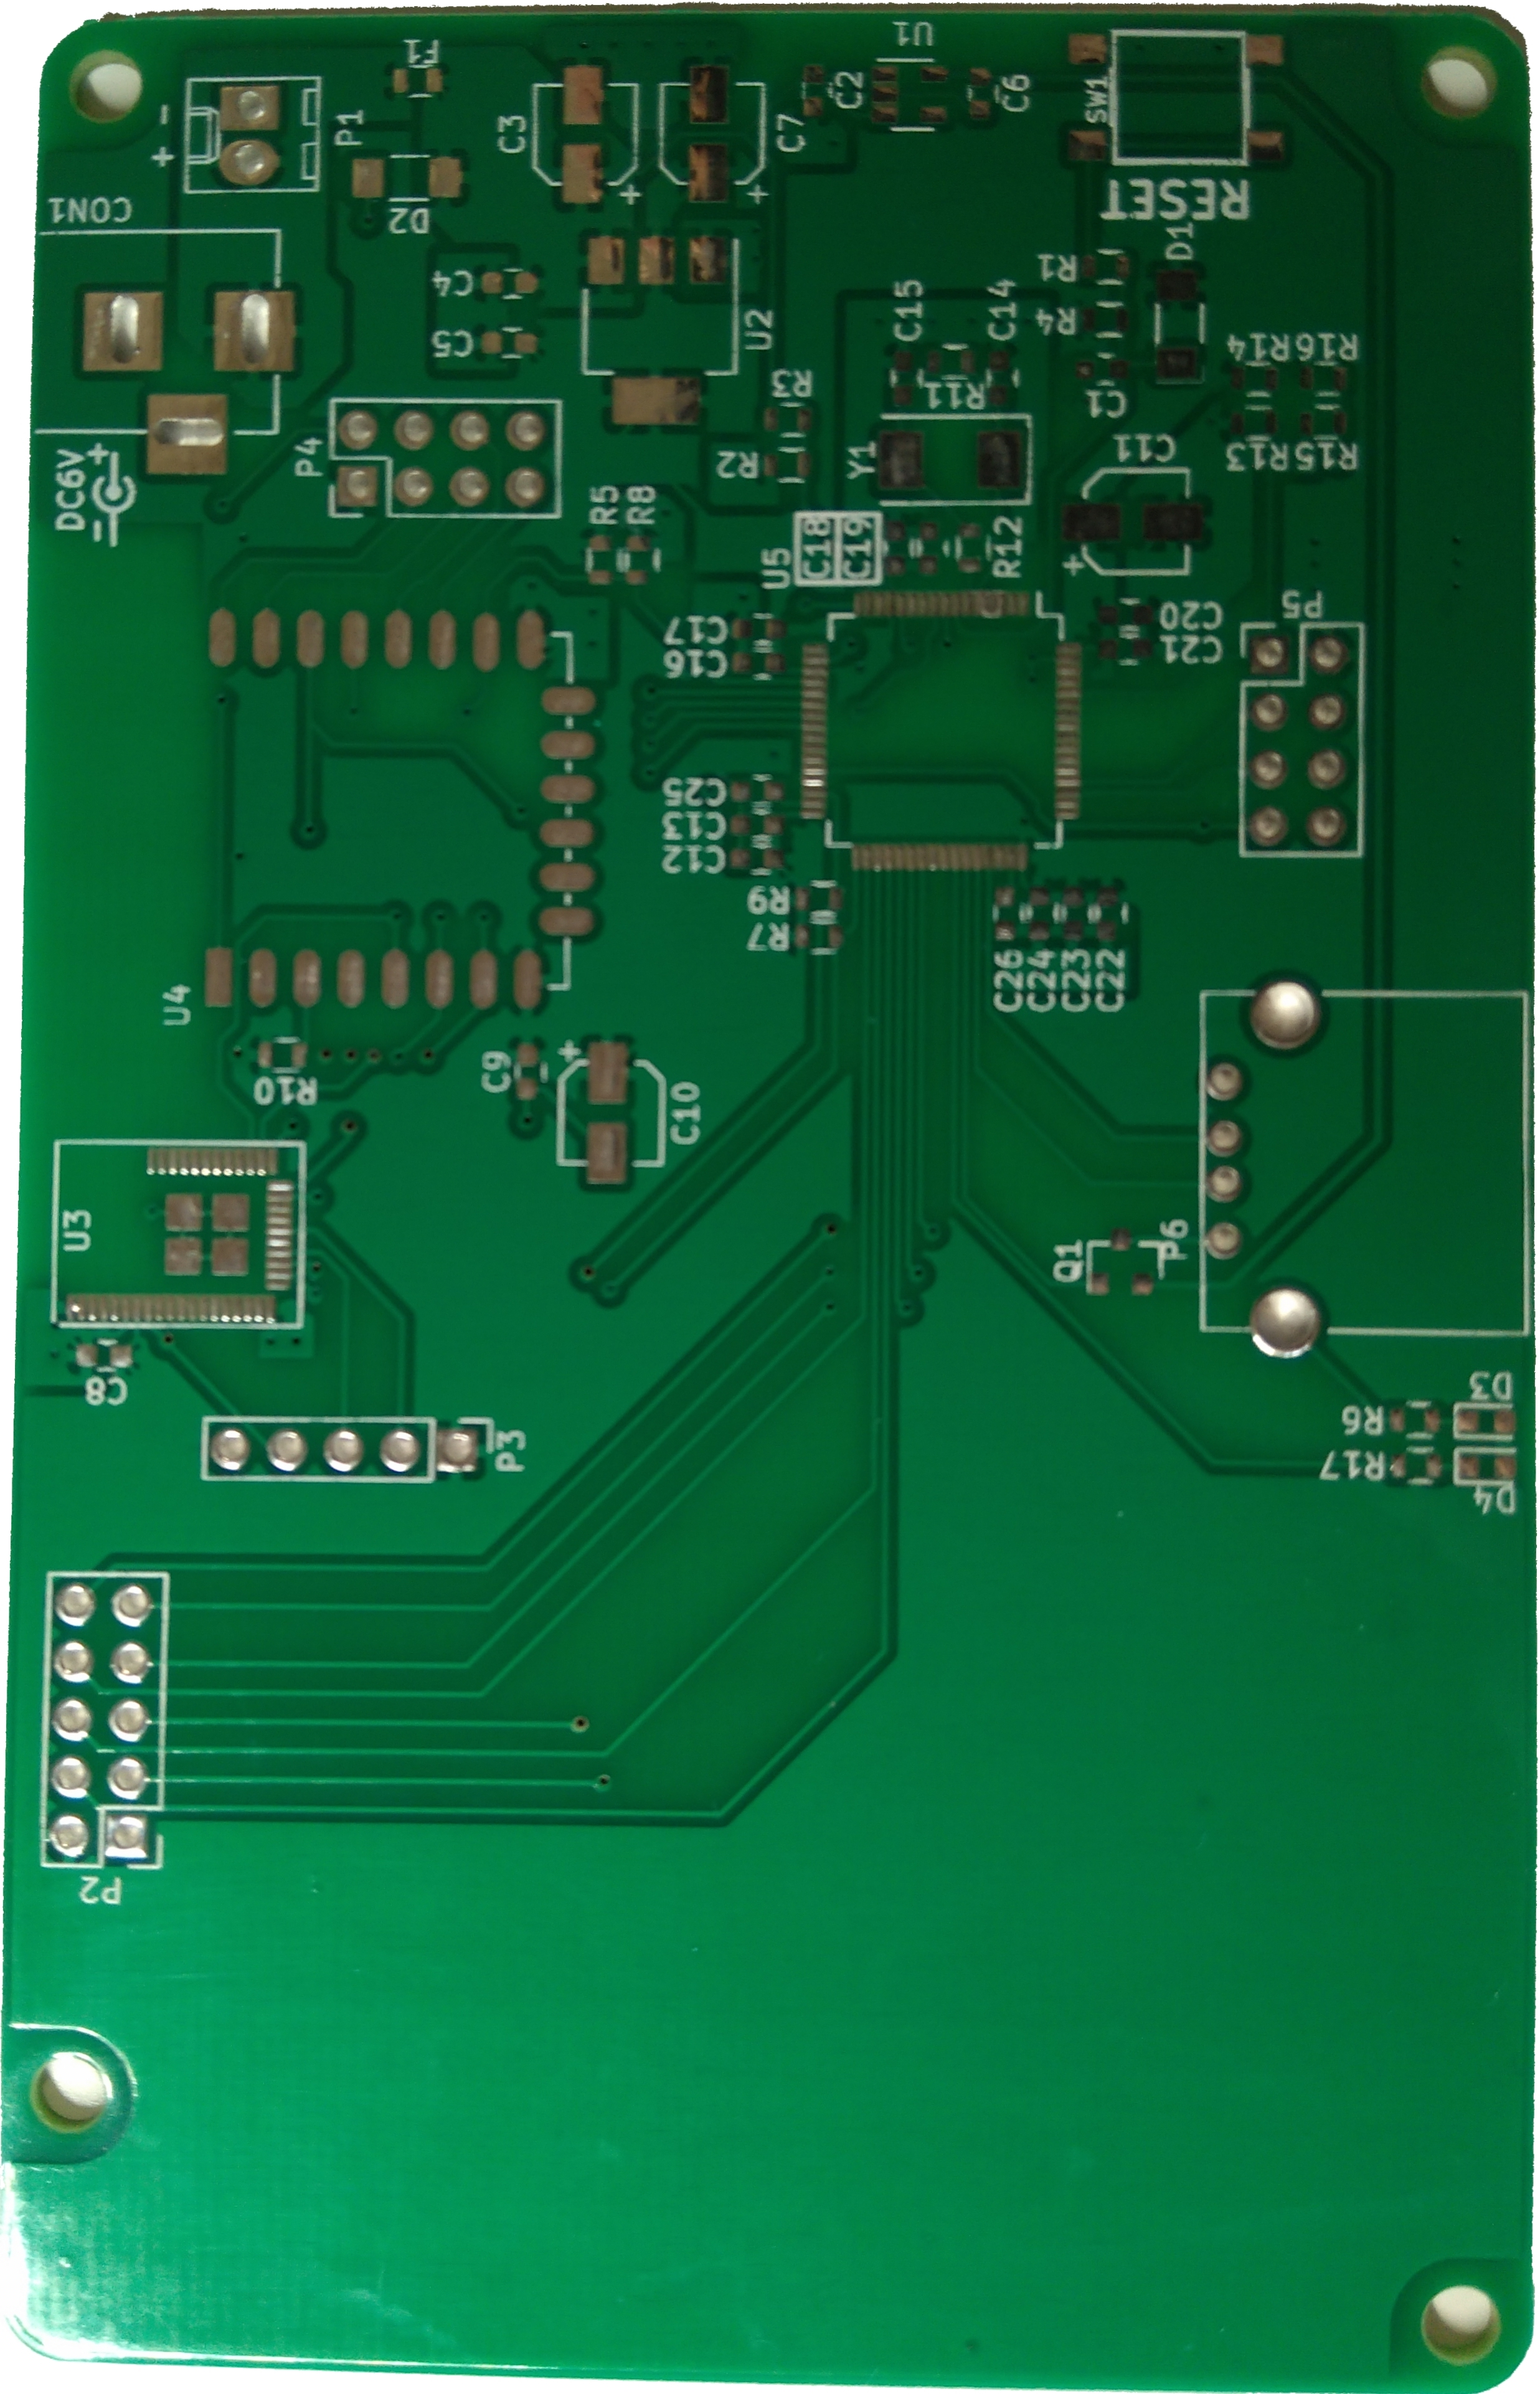
\includegraphics[width=8cm]{PCB_Front_real}
    \caption{Impresión final}
    \label{fig:PCB_Front_real}
  \end{subfigure}
  \caption{\textit{Layout} en KiCad (a) e impresión final (b) de la capa superior}
  \label{fig:PCB_Front_completa}
\end{figure}

El resultado es bastante positivo. Al haberse respetado todas las restricciones de diseño impuestas por el fabricante, no hay ningún cortocircuito y todas las pistas se han impreso correctamente.

Aquellas zonas en las que no hay conductor en ninguno de los planos aún presenta un soporte físico de fibra de vidrio para dotar de consistencia a la placa.

La \textbf{serigrafía} que acompaña a los componentes así como la generada manualmente se aprecia con mayor \textbf{claridad} incluso que en la previsualización generada por KiCad.

\clearpage

\begin{figure}[h]
  \begin{subfigure}[b]{8cm}
   	\centering
    \includegraphics[height=8cm, angle = 90]{PCB_Back}
    \caption{\textit{Layout} en KiCad.}
    \label{fig:PCB_Back}
  \end{subfigure}
  \hfill
  \begin{subfigure}[b]{8cm}
  	\centering
    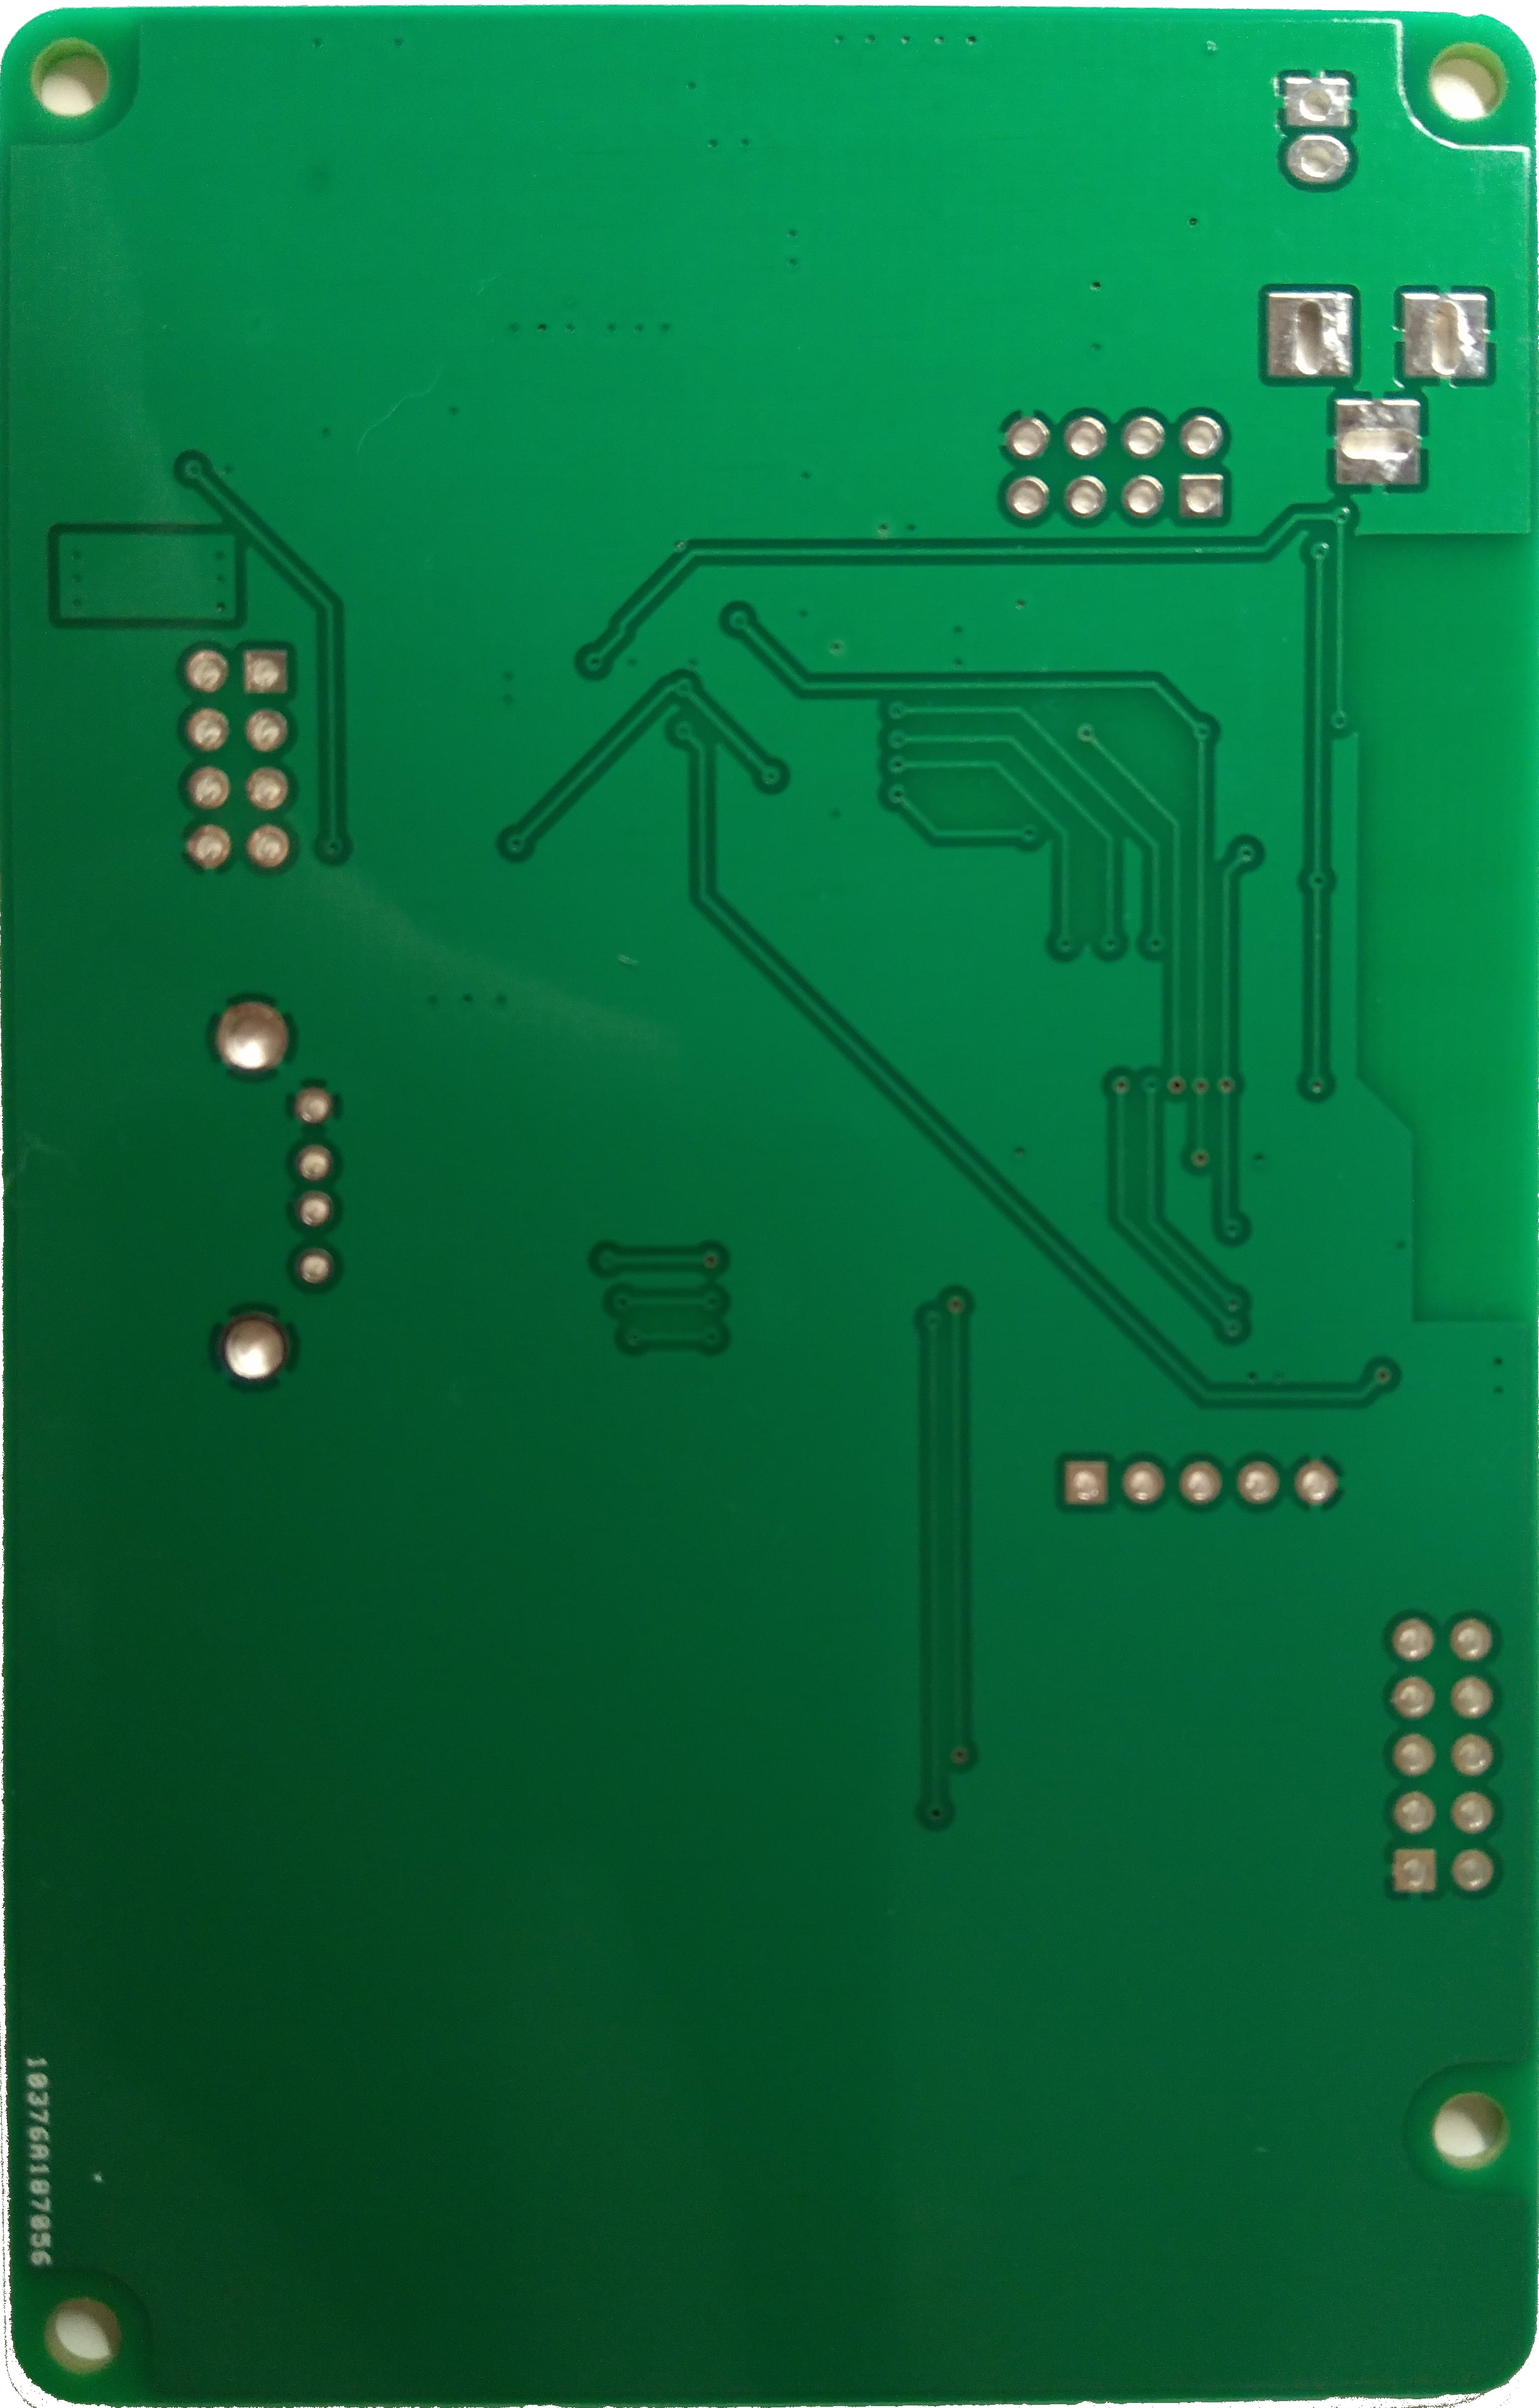
\includegraphics[width=8cm]{PCB_Back_real}
    \caption{Impresión final}
    \label{fig:PCB_Back_real}
  \end{subfigure}
  \caption{\textit{Layout} en KiCad (a) e impresión final (b) de la capa inferior}
  \label{fig:PCB_Back_completa}
\end{figure}

Como se puede observar, la impresión real se encuentra en \textbf{modo espejo} con el \textit{layout} de KiCad de la capa inferior. Este fenómeno ocurre debido a  al trabajar con la capa inferior en KiCad se mantiene la \textbf{vista cenital} y las capas superiores simplemente no se \textbf{renderizan}. Con esto se consigue facilitar el proceso de diseño, no sólo por mantener un punto de referencia constante, sino porque al trazar pistas se puede pasar con comodidad entre unas capas y otras sin tener que cambiar el modo de vista.

\subsection{Previsualización 3D vs resultado final\label{sec:Modelo_3D}}

Normalmente el \textit{footprint} de un componente incluye una serigrafía que delimita la zona de la placa que ocupará, garantizando que dos componentes cuya serigrafía no se solape no causarán problemas en el montaje final.

Por desgracia, esto no siempre se cumple y en ocasiones puede ocurrir que dos componentes procedentes de una librería poco fiable contengan información errónea. 

\clearpage

Para minimizar las posibilidades de error y asegurarse que el resultado final será el deseado KiCad permite realizar una \textbf{representación 3D} de todos los componentes así como su posición relativa en la placa.


\begin{figure} [h]
    \centering
    \includegraphics[width=15cm]{PCB_3D}

    \includegraphics[width=15cm]{PCB_3D_real}
    \caption{Modelo 3D del sistema (arriba) y placa final (abajo)}
    \label{fig:Comparativa_PCB_final}
\end{figure}

En la figura \ref{fig:Comparativa_PCB_final} se puede comprobar que, efectivamente, la \textbf{representación 3D proyectada}  durante la fase de diseño ha resultado ser \textbf{fiel al producto final} obtenido.
